\documentclass[12pt]{article}
\usepackage{graphicx}
\usepackage{amsmath,amsfonts,amssymb,geometry}
\usepackage{natbib}
\usepackage{dcolumn}
\usepackage{float}
\usepackage{booktabs, threeparttable}
\bibliographystyle{aer}
\geometry{a4paper, margin=1in}
\title{Sketch for Empirical Analysis}
\author{Zhiyao (Yao) Ma}
\date{\today}

\begin{document}
\maketitle

\section{Empirical Evidence}

\noindent Our empirical analysis integrates farmers' trading records, subjective market expectations, and objective measures of time-varying competition to examine the role of storage in improving smallholder welfare. Specifically, it investigates how storage enables inter-temporal arbitrage, allowing farmers to sell in more competitive farm-gate oligopsonistic markets—an aspect often overlooked in smallholder market research.

Existing observational data are insufficient, as micro-surveys typically capture post-trade information (e.g., transaction prices, storage volumes) but lack measures of temporal market competitiveness, such as buyer visits and price offer frequency after harvest. Thus, a survey-based approach is necessary to assess how storage decisions and local procurement market structures shape farmer bargaining power.

This study surveys both farmers and middlemen in a Central China county where Fuji apple cultivation dominates. Given the region's reliance on a single cash crop and the strategic role of cold storage in marketing decisions, it provides an ideal setting to analyze the interaction between storage and market competition.


%------------------------------------------------------%
\subsection{Field Site: a County in Central China}
\noindent Yanchang County, Shaanxi province, China (see Figure \ref{Figure: Yanchang}), serves as an ideal location to study farmers' marketing and storage decisions. The county is home to numerous small-scale farmers who heavily rely on a single cash crop, primarily Fuji apples, for their livelihoods. Each village within the county possesses a central market where farmers sell their produce, attracting middlemen and traders. Cold storage facilities are also available for farmers to rent or purchase, providing them with access to these inputs. In 2024, the fruit storage facilities in the entire county can accommodate up to 180,000 tons of fresh apples, with most of the capacity utilized in a given year.

\begin{figure}[thp]
\centering
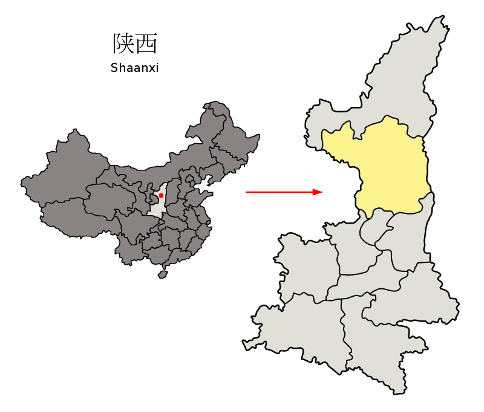
\includegraphics[width=0.6\textwidth]{figures/yanchang_map.png}
\caption{Location of Yanchang County in China}
\label{Figure: Yanchang}
\end{figure}

The apple farmers in Yanchang County predominantly cultivate late-maturing Fuji apples, which constitute approximately 85-90\% of the production. Some farmers also grow mid-maturing apples (5-10\%) and early-maturing apples (around 5\%). Farm-gate prices range from 2.5 to 12 yuan/kg and can be checked regularly. The yield per acre does not significantly differ among the three apple varieties.

Although there are over 260 villages in the county, the average number of fruit storage facilities is slightly over 100, meaning that there is less than one facility per administrative village. Cold storage facilities owned by apple growers in Yanchang County can be classified into two types: small-scale facilities capable of storing up to 50 tons and medium-sized facilities with a capacity of up to 500 tons. According to the government report, only 1.3\% of farmers possess their own small-scale cold storage facilities. However, many farmers rent cold storage facilities established by the township and large merchants. It is worth noting that the quality of fruit storage facilities constructed by township governments is subpar compared to those built by farmers themselves. Farmers contribute 60\% of the investment, while the government subsidizes the remaining 40\%.

Farmers in Yanchang County who do not adopt cold storage facilities have to sell their harvest within a month. On the other hand, farmers using cold storage facilities need to consider various factors and market conditions, including the time-varying competition among traders. With cold storage, they can market their produce until April or May of the following year without significant deterioration. Furthermore, they are not necessarily limited to selling to middlemen but also sometimes do retail selling to consumers directly, as storage facilities grant them temporal flexibility to find more potential buyers.


%------------------------------------------------------%
\subsection{Data}
\subsubsection{Sampling Procedure}
\noindent This study employs empirical tests using data collected from two rounds of a survey of 615 smallholder apple growers in Yanchang County, Central China, covering the 2024/2025 agricultural season. With Institutional Review Board (IRB) approval, the survey was conducted between October 10, 2024, and December 13, 2024. Given that the harvest season for Fuji apples in Central China concludes in mid-to-late October, followed immediately by the lean season, this period provides a relevant timeframe to analyze the evolving market conditions faced by farmers.

The survey was conducted in collaboration with the Yanchang-County Women's Federation (YWF), an organization responsible for public welfare and rural development in Yanchang County. In coordination with the Yanchang County Agricultural Bureau, the YWF facilitated access to micro-level data on apple growers, enabling a structured sampling approach. A one-layer stratified random sampling method was employed based on geographical location. Yanchang County consists of one urban subdistrict and seven rural towns. To ensure representativeness, the Yanchang County Agricultural Bureau determined the approximate sampling proportion for each town based on the number and density of fruit farmers (30\%:15\%:15\%:15\%:10\%:5\%:5\%:5\%). Following these proportions, smallholder apple-growing households were randomly selected from rosters provided by administrative villages within each town.

For the purpose of this study, smallholder apple growers are defined as farmers who cultivate no more than 50 mu of land and derive at least 90\% of their agricultural income from apple production. Additionally, to maintain sufficient sample sizes across towns, a minimum of 10 participating apple growers was ensured in each town, though no minimum was imposed at the village level.

The survey targeted farmers whose primary source of income is derived from growing red Fuji apples. The interviews were conducted with the household head, except in cases where the household head was elderly and no longer part of the active labor force. In such instances, the survey was conducted with the primary labor force member of the household.


\subsubsection{Farmers' Storage Usage and Procurement Competitiveness}
\noindent This study examines apple growers' cold storage usage and marketing timing decisions as key dependent variables. First, we define \texttt{Storage-Usage-Binary}, a binary indicator equal to 1 if a farmer used cold storage at harvest and 0 otherwise. Second, \texttt{Storage-Usage-Type} categorizes storage choices into four groups: \textit{Not\_use}, and three storage options—\textit{Rent\_large}, \textit{Rent\_small}, or \textit{Self\_built}—each indicating some form of cold storage usage. Third, \texttt{Time-to-Sell} measures the delay between harvest and sale, effectively representing storage duration. Sales occurring in October are classified as 1–4 weeks post-harvest, November as 5–8 weeks, and so forth, yielding interval-censored data with four predefined selling-time intervals: 1–4, 5–8, 9–12, and 13–28 weeks. Figure \ref{Figure: selling weeks distribution} illustrates the distribution of selling weeks by storage type.

\begin{figure}[H]
\centering
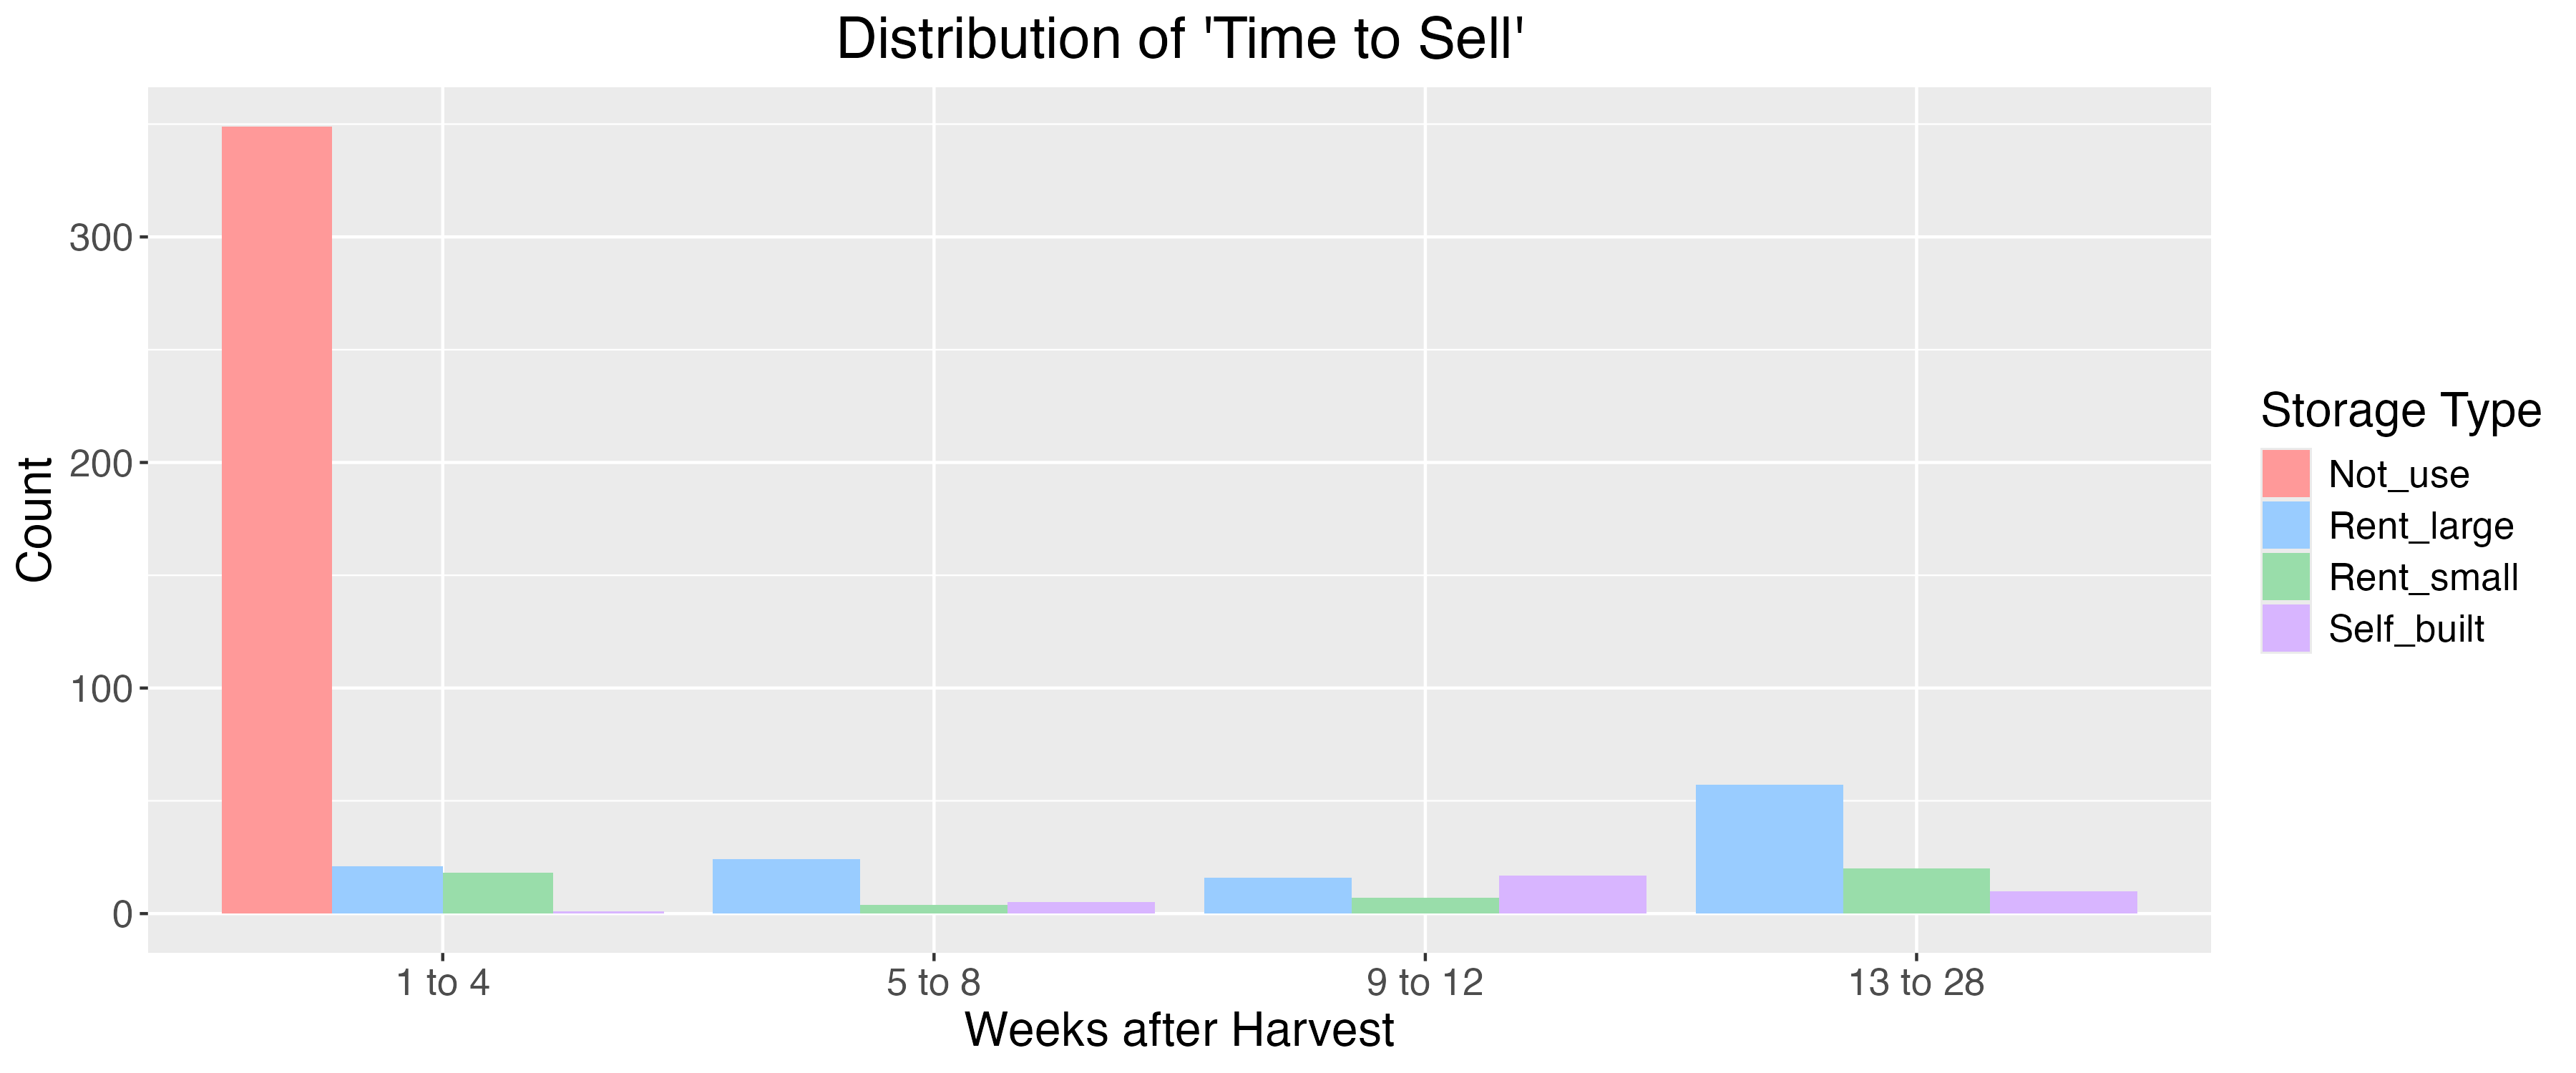
\includegraphics[width=1\textwidth]{figures/selling_weeks_distribution.png}
\caption{Distribution of Selling Weeks by Storage Type}
\label{Figure: selling weeks distribution}
\end{figure}

To capture inter-temporal variations in oligopsony power among buyers, farmers were asked to report:
\begin{enumerate}
    \item Their subjective assessment of buyer competition at harvest time (\texttt{Subjective buyer competitiveness}, measured on a 1–5 scale);
    \item Their expectations regarding changes in the number of traders over the subsequent three months (October 2024 onward), recorded as \texttt{Expect more buyers} and \texttt{Expect fewer buyers}.
\end{enumerate}

Additionally, the survey collected data on farmers' total annual agricultural income, production costs, storage expenses, and demographic characteristics to assess welfare implications.

To complement these farmer-level insights with market-level dynamics, a buyer survey was conducted in December 2024. This survey targeted 15 buyers, including the top five most influential local traders, and collected data on:
\begin{enumerate}
    \item The specific villages each buyer visited during the October harvest;
    \item The cold storage facilities from which they had procured apples over the preceding two months.
\end{enumerate}
These responses allow us to construct an objective measure of buyer concentration and inter-temporal competition. Inspired by \cite{macchiavello2021competition}, who used the number of mills within a 10 km radius as a competition metric, we define \texttt{Number of buyers} as the count of traders visiting each village post-harvest.

%------------------------------------------------------%
\subsection{Descriptive Statistics}
\noindent The final dataset comprises 549 smallholder apple-growing households. Among them, 200 farmers used cold storage in the 2024–2025 agricultural year, with 33 storing apples in self-built facilities, 49 using small-scale commercial storage, and 118 opting for large-scale commercial storage. Figure \ref{Figure: pie and radar chart} presents the distribution of storage usage types.

\begin{figure}[H]
\centering
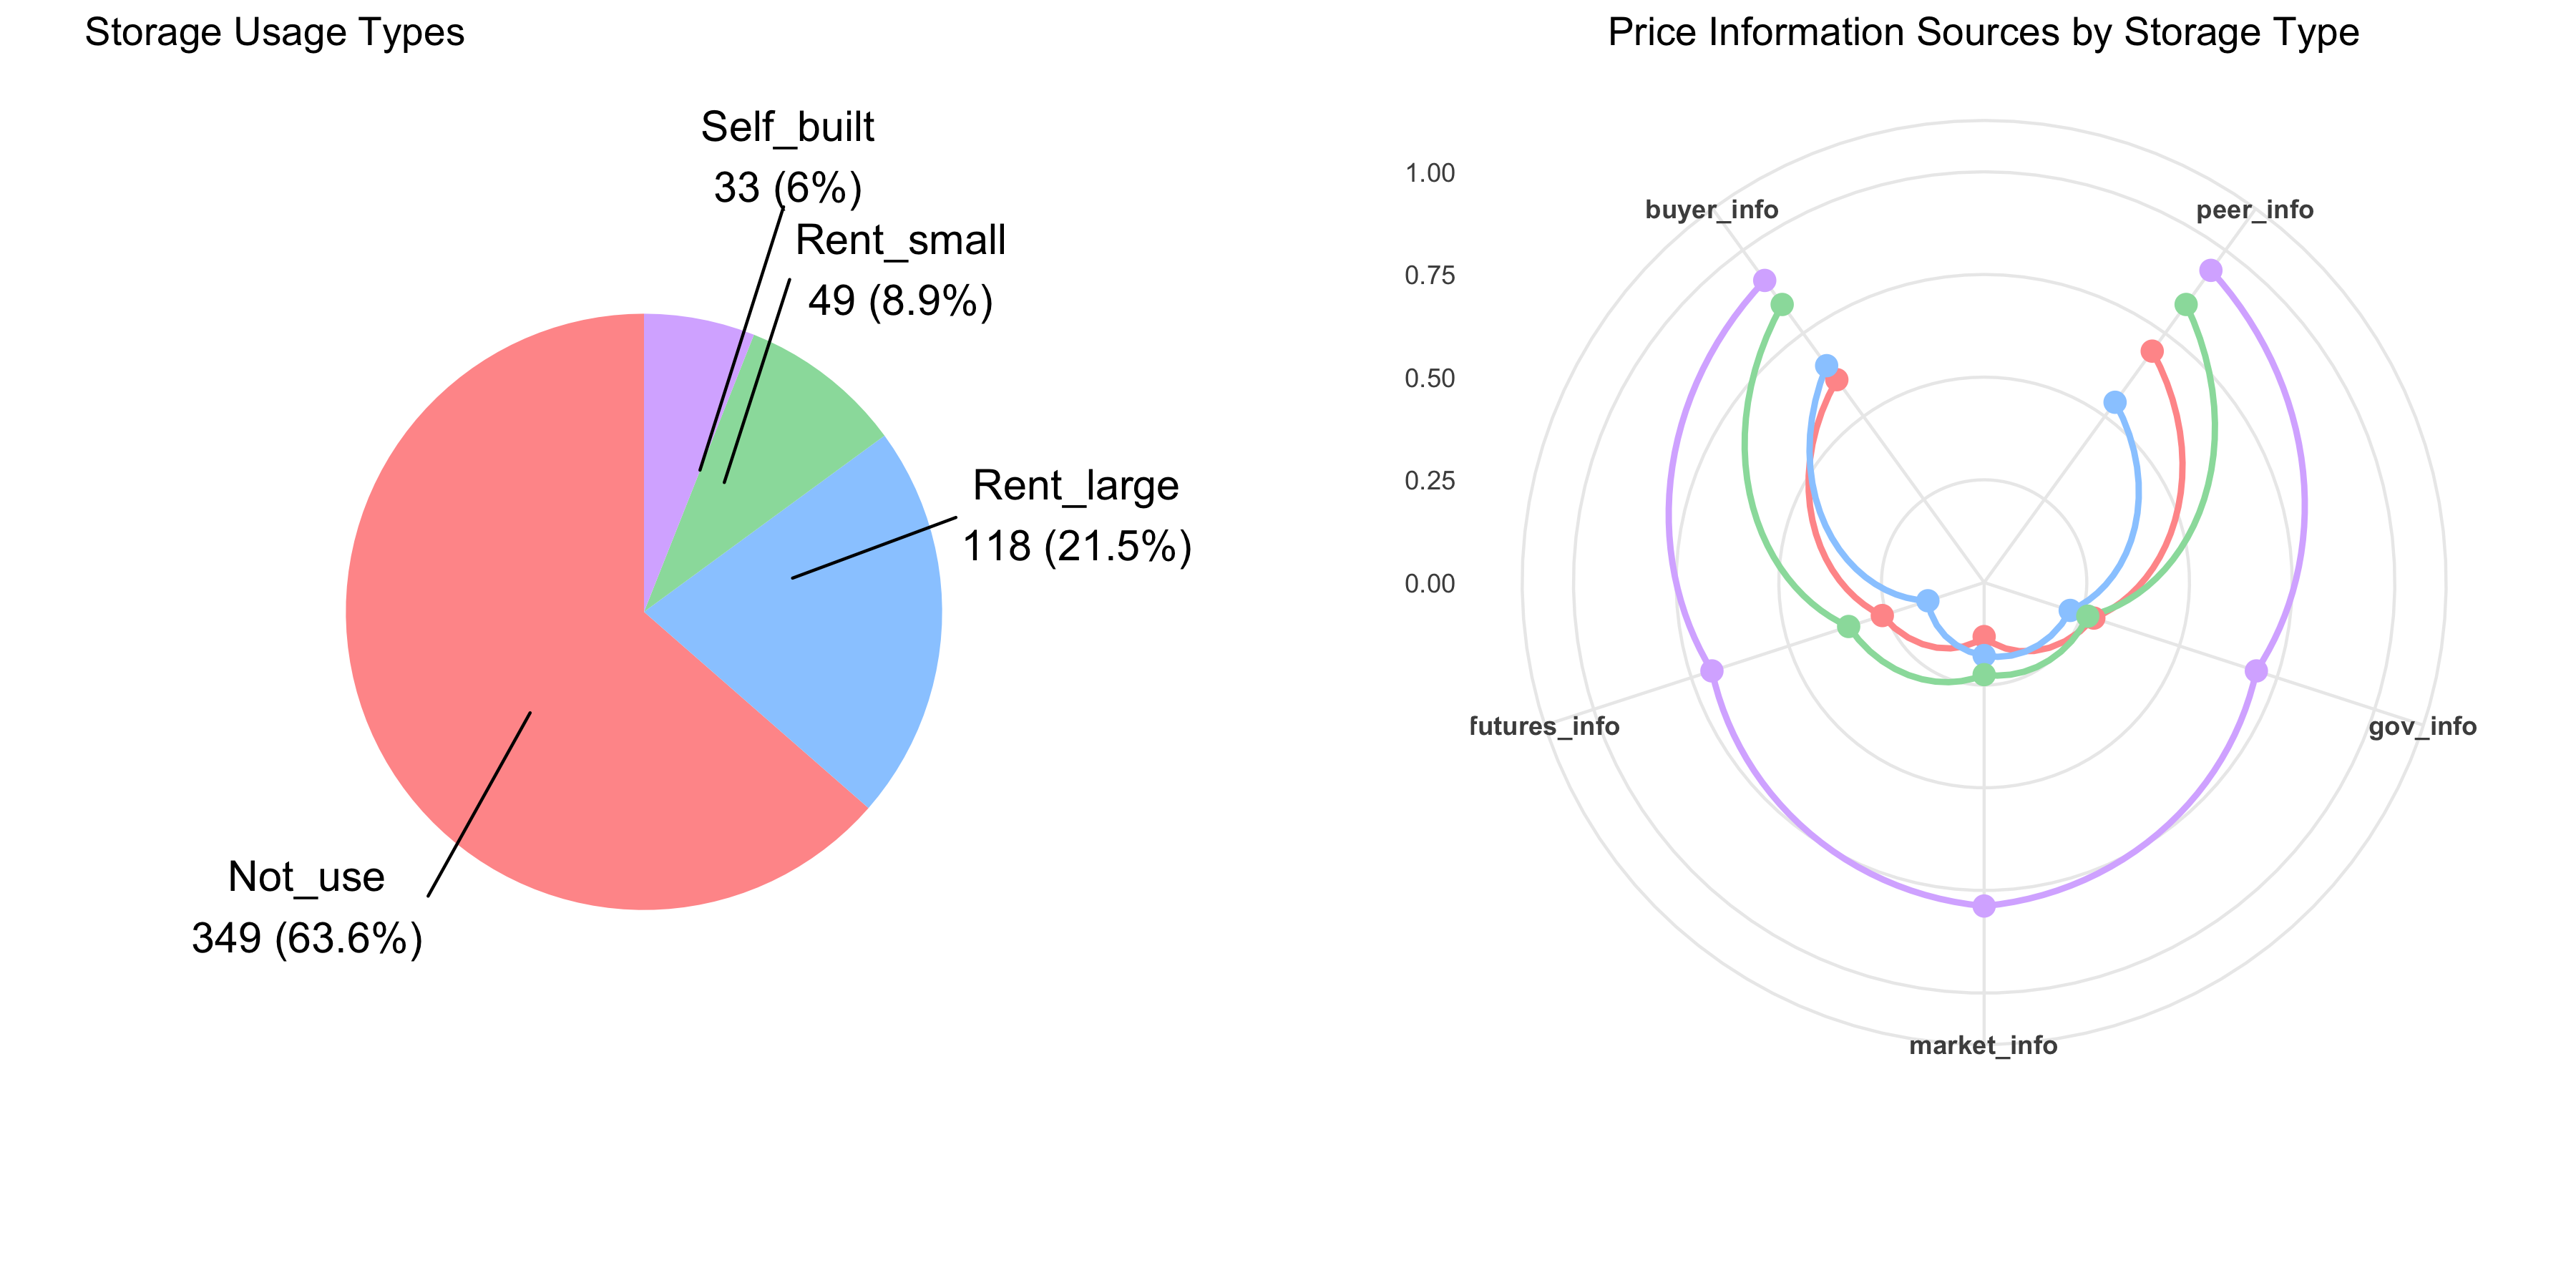
\includegraphics[width=1\textwidth]{figures/storage_usage_analysis_soft_colors.png}
\caption{Distribution of Storage Usage Types and Their Price Information Sources}
\label{Figure: pie and radar chart}
\end{figure}

These 200 storage users form a key sub-sample for analyzing storage behavior. Table \ref{tab: summary statistics} reports summary statistics for both the full sample and this sub-sample, covering key variables such as \texttt{Number of buyers} at harvest, \texttt{Subjective buyer competitiveness}, and farmers' expectations of future buyer competition (Panel E), alongside additional survey variables employed in this study. 







%------------------------------------------------------%
%------------------------------------------------------%






\newpage
\subsection{Analysis by Specific Storage Types}

\begin{table}[H]
\centering
\caption{Summary Statistics by Storage Usage}
\label{tab: summary statistics}
\resizebox{\textwidth}{!}{%
\begin{tabular}{lccccc}
\toprule
 & \multicolumn{2}{c}{Storage Users} & \multicolumn{2}{c}{Non-Users} & Difference \\
\cmidrule(lr){2-3} \cmidrule(lr){4-5}
Variable & Mean & SD & Mean & SD & t-statistic \\
\midrule
\multicolumn{6}{l}{\textbf{Panel A: Farmer Demographics}} \\
Age (years) & 56.87 & (9.57) & 60.35 & (9.63) & -4.09*** \\
Household size (persons) & 2.71 & (1.21) & 2.58 & (1.10) & 1.24 \\
Labor size (persons) & 1.74 & (0.71) & 1.60 & (0.66) & 2.20** \\
Highest education (level) & 1.96 & (0.67) & 1.81 & (0.76) & 2.35** \\
Family ever village leader (0/1) & 0.24 & (0.43) & 0.06 & (0.24) & 5.37*** \\
Liquidity constrained (0/1) & 0.15 & (0.36) & 0.16 & (0.37) & -0.17 \\
\addlinespace
\multicolumn{6}{l}{\textbf{Panel B: Production and Consumption}} \\
Apple yield (tons) & 11.08 & (7.56) & 11.68 & (14.12) & -0.64 \\
Land size (acre) & 2.60 & (1.70) & 1.72 & (0.99) & 6.69*** \\
Bad apple ratio & 2.31 & (1.20) & 2.02 & (1.18) & 2.78*** \\
Apple income (USD) & 10127.22 & (6108) & 8289 & (6465) & 3.32*** \\
Total income (USD) & 10919 & (6445) & 8990 & (7334) & 3.21*** \\
Labor cost (USD) & 1911 & (1593) & 1343 & (1258) & 4.33*** \\
Family consumption (USD) & 7117 & (8899) & 5059 & (3869) & 3.11*** \\
\addlinespace
\multicolumn{6}{l}{\textbf{Panel C: Storage and Risk-Related Factors}} \\
Car/truck ownership (0/1) & 0.14 & (0.35) & 0.04 & (0.20) & 3.61*** \\
Natural disaster insurance (0/1) & 0.35 & (0.48) & 0.33 & (0.47) & 0.49 \\
Price insurance (0/1) & 0.62 & (0.49) & 0.65 & (0.48) & -0.78 \\
CRRA adjusted (coef) & 0.09 & (0.37) & 0.36 & (0.45) & -7.75*** \\
Storage in village (0/1) & 0.38 & (0.49) & 0.20 & (0.60) & 3.74*** \\
Far to small storage (0/1) & 0.52 & (0.50) & 0.79 & (0.41) & -6.71*** \\
Far to large storage (0/1) & 0.89 & (0.32) & 0.91 & (0.28) & -1.07 \\
Storage for wider marketing (0/1) & 0.88 & (0.33) & 0.30 & (0.46) & 16.90*** \\
Storage as bargaining tool (0/1) & 0.80 & (0.40) & 0.29 & (0.46) & 13.79*** \\
\addlinespace
\multicolumn{6}{l}{\textbf{Panel D: Marketing}} \\
Highest price per pound (USD/lb) & 0.41 & (0.09) & 0.38 & (0.10) & 3.94*** \\
Good price per pound (USD/lb) & 0.40 & (0.08) & 0.37 & (0.10) & 3.29*** \\
WeChat selling (0/1) & 0.15 & (0.36) & 0.00 & (0.00) & 6.04*** \\
Relational selling (0/1) & 0.12 & (0.33) & 0.14 & (0.35) & -0.78 \\
Contract selling (0/1) & 0.40 & (0.49) & 0.26 & (0.44) & 3.32*** \\
\addlinespace
\multicolumn{6}{l}{\textbf{Panel E: Market Competitive Conditions}} \\
Expect more buyers (0/1) & 0.46 & (0.50) & 0.06 & (0.23) & 10.75*** \\
Expect fewer buyers (0/1) & 0.16 & (0.39) & 0.19 & (0.39) & -0.90 \\
Number of buyers at harvest (count) & 3.83 & (2.45) & 3.12 & (1.91) & 3.51*** \\
Subjective buyer competitiveness (1/5) & 2.92 & (0.84) & 3.06 & (0.69) & -2.08** \\
\hline
\hline
Observations & 200 & & 349 & & 549 \\
\bottomrule
\end{tabular}% 
} % End of resizebox 
\begin{tablenotes} 
\item \textit{Notes:} The table presents means and standard deviations (in parentheses) for each variable by group. T-statistics from two-sample t-tests are reported to indicate statistical significance of differences between groups. Significance levels are denoted by asterisks: * p$<$0.1, ** p$<$0.05, *** p$<$0.01. In addition, monetary values have been converted from Chinese Yuan (RMB) to US Dollars (USD), land area from mu to acres, and apple prices from RMB/kg to USD/pound using appropriate conversion rates. 
\end{tablenotes} 
\end{table}



\begin{figure}[H]
\centering
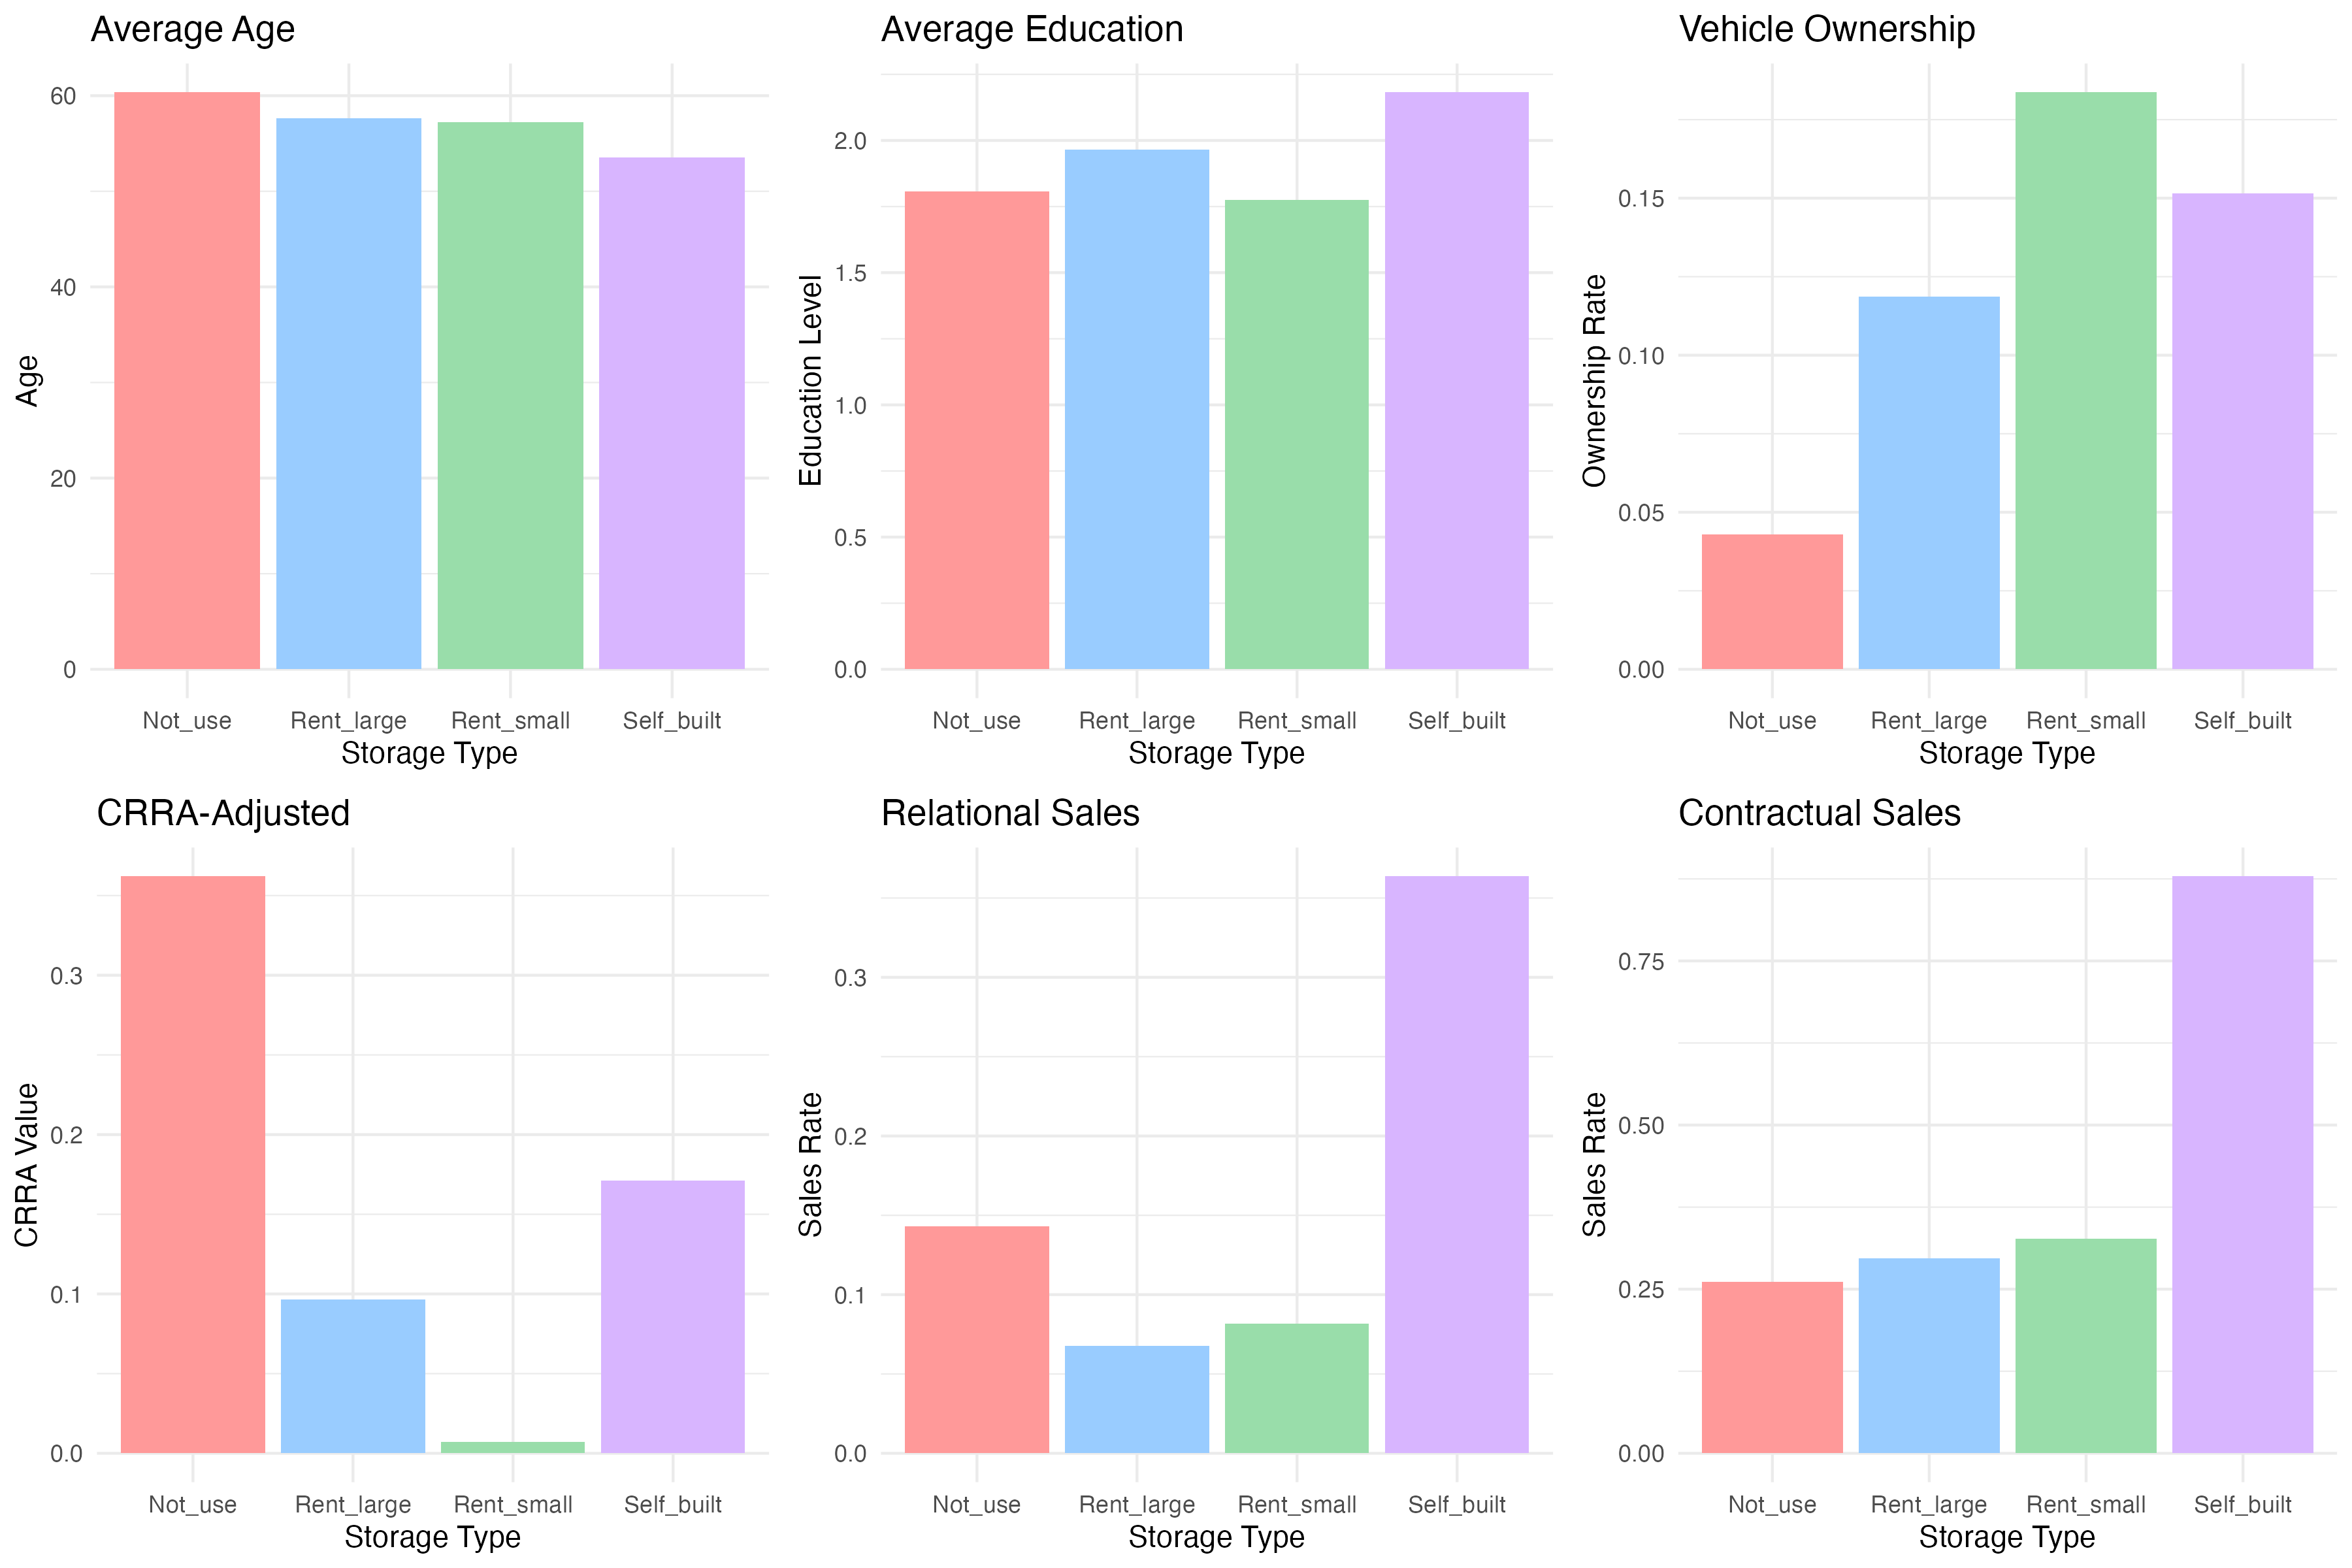
\includegraphics[width=1\textwidth]{figures/combined_storage_metrics.png}
\caption{Demographics by Storage Type}
\label{Figure: Demographics by Storage Type}
\end{figure}

\begin{figure}[H]
\centering
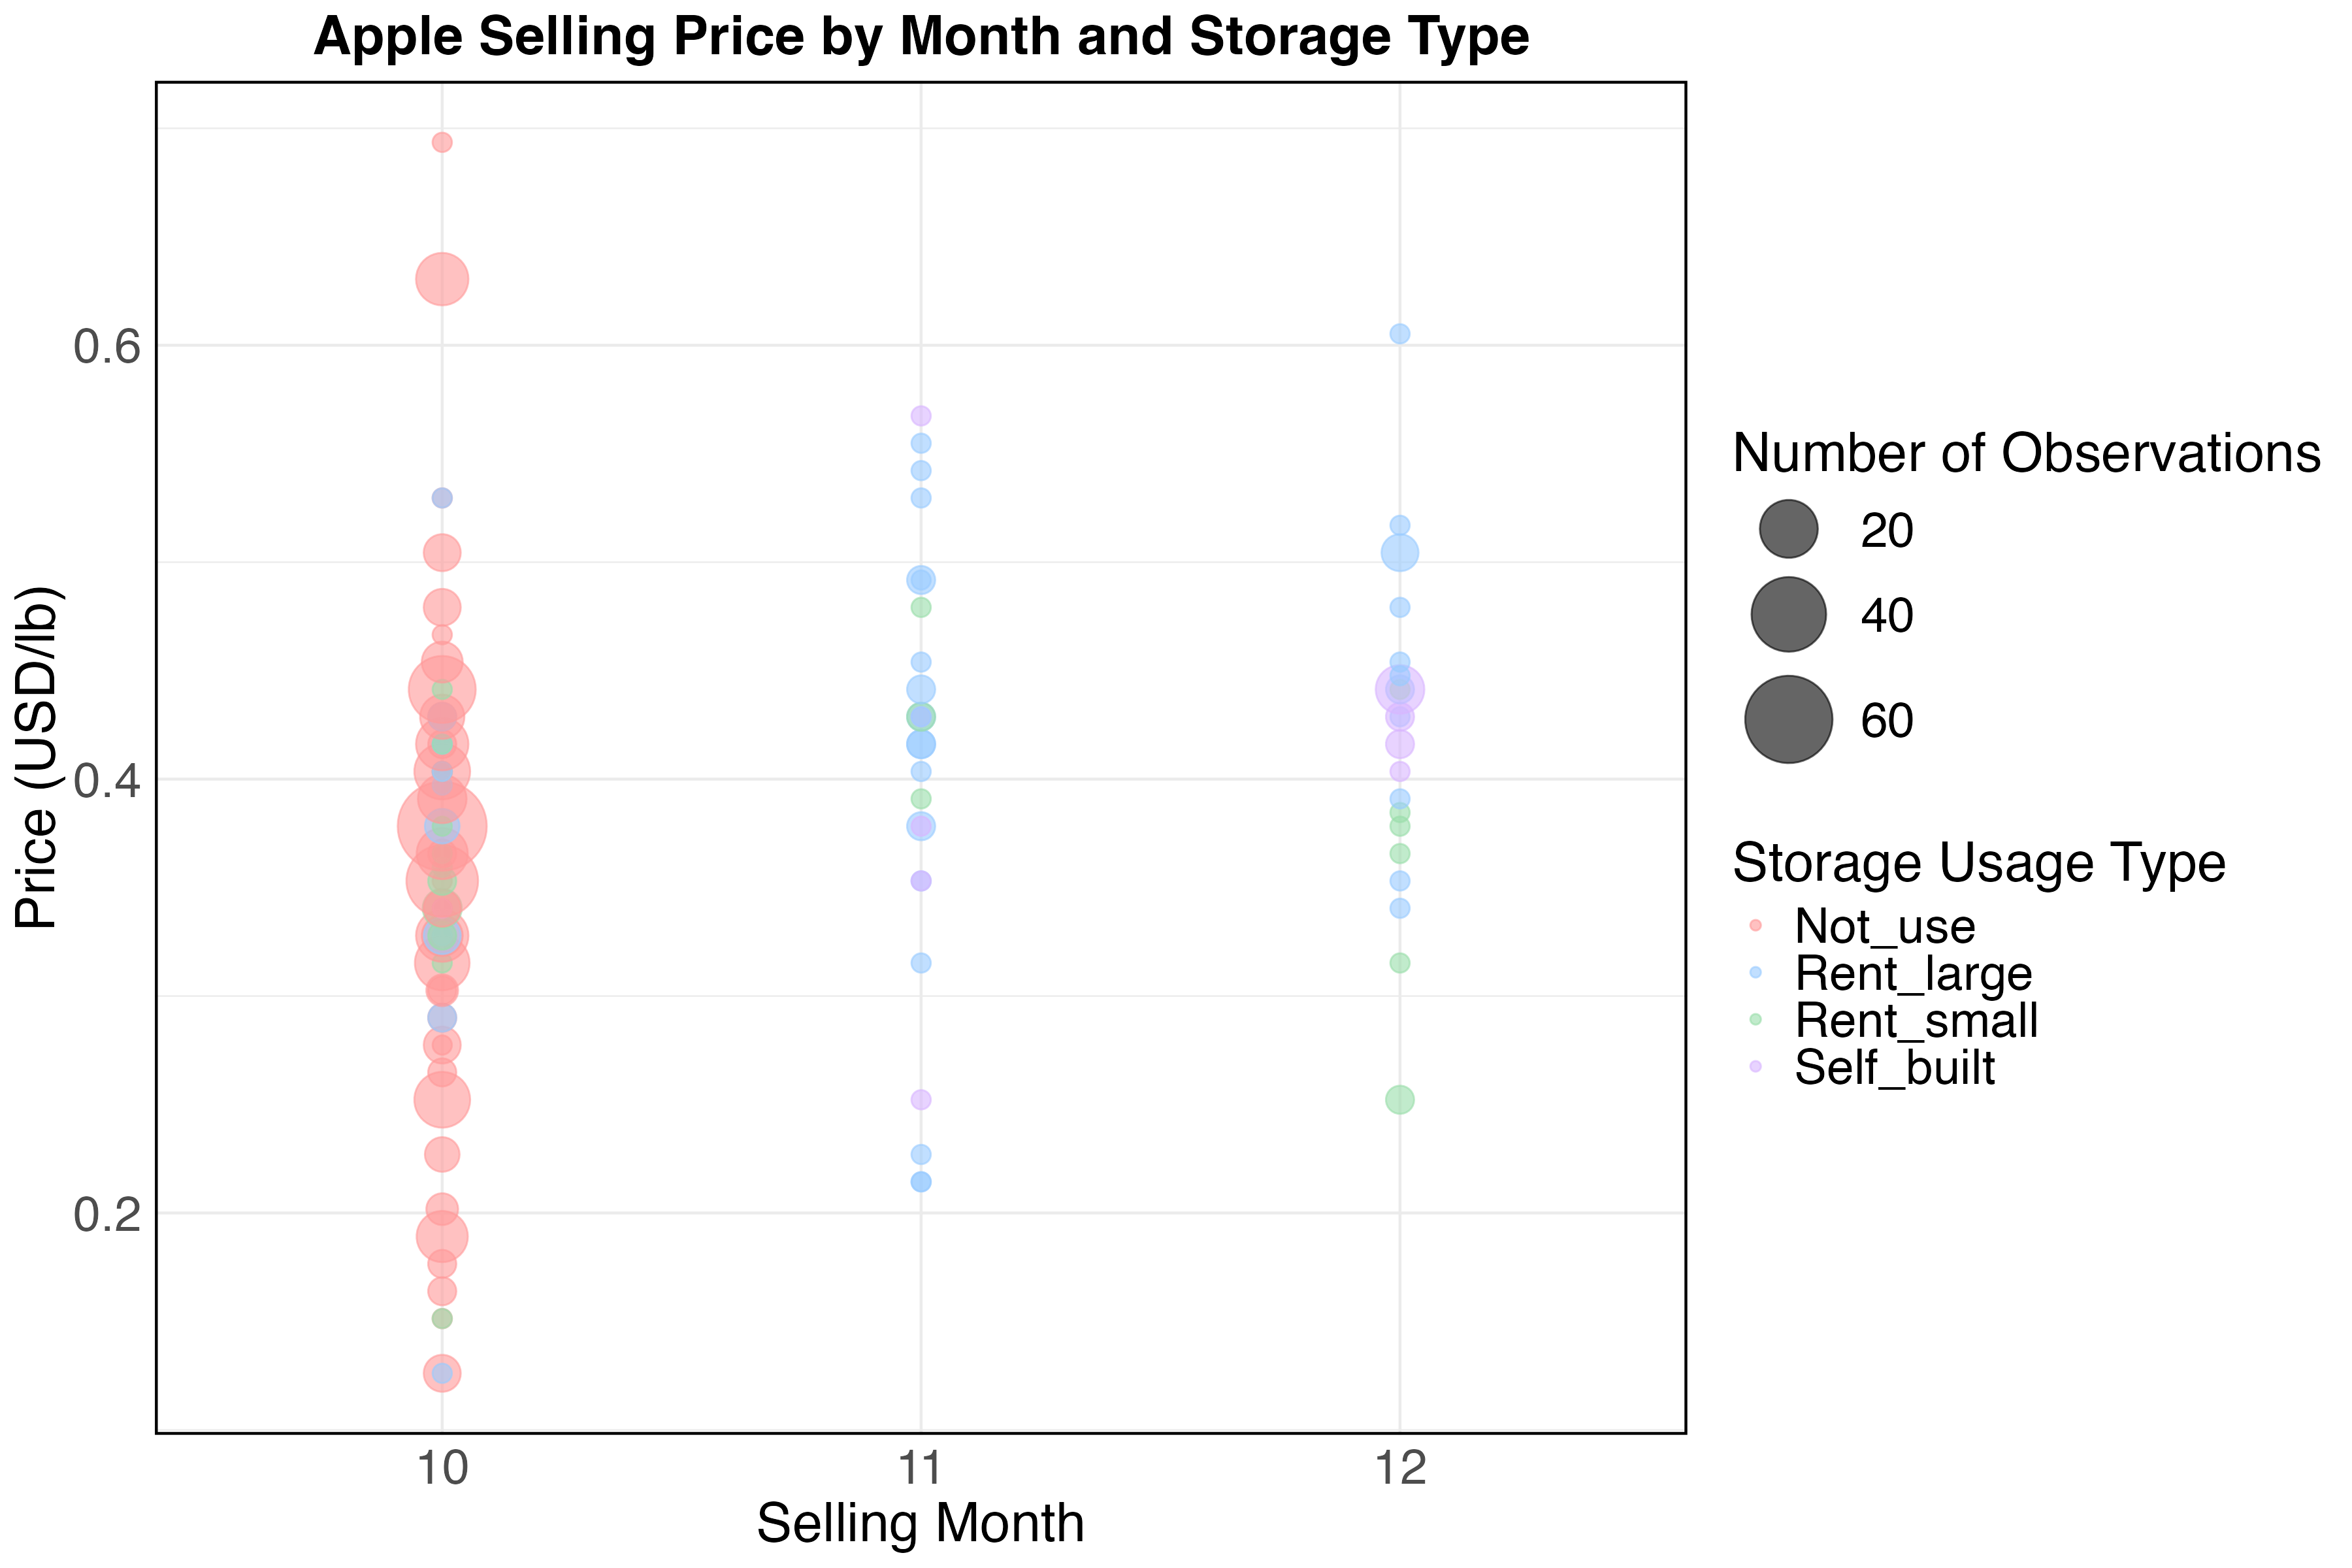
\includegraphics[width=1\textwidth]{figures/apple_price_bubble_plot.png}
\caption{Apple Selling Price by Month and Storage Type}
\label{Figure: selling price bubble}
\end{figure}




\begin{table}[H]
    \centering
    \footnotesize
    \begin{threeparttable}
        \caption{Reasons for Not Using Storage Facilities}
        \label{tab:non_storage_reasons}
        \begin{tabular}{lc}
            \toprule
            \textbf{Reason} & \textbf{Percentage} \\
            \midrule
            High Storage Costs & 22.92\% \\
            Produce has been pre-ordered & 8.02\% \\
            Cannot sell high later & 60.75\% \\
            Too risky & 28.65\% \\
            \bottomrule
        \end{tabular}
        \begin{tablenotes}
            \item \textit{Notes:} This table presents the reasons provided by the 349 farmers who do not use storage facilities, expressed as percentages of total non-storage farmers.
        \end{tablenotes}
    \end{threeparttable}
\end{table}




\newpage
\subsection{Buyers' Competitiveness at Harvest on Binary Storage Decisions}

% Table created by stargazer v.5.2.3 by Marek Hlavac, Social Policy Institute. E-mail: marek.hlavac at gmail.com
% Date and time: Wed, Sep 24, 2025 - 19:45:19
\begin{table}[H] \centering 
  \caption{Logistic Regression Results} 
  \label{tab: binary storage ~ buyers' competition at harvest} 
\footnotesize 
\begin{tabular}{@{\extracolsep{5pt}}lccc} 
\\[-1.8ex]\hline 
\hline \\[-1.8ex] 
 & \multicolumn{3}{c}{\textit{Dependent variable:}} \\ 
\cline{2-4} 
\\[-1.8ex] & \multicolumn{3}{c}{Storage Usage (Binary)} \\ 
 & Model 1 & Model 2 & Model 3 \\ 
\\[-1.8ex] & (1) & (2) & (3)\\ 
\hline \\[-1.8ex] 
 Number of Buyers & 0.004 &  & 0.45$^{***}$ \\ 
  & (0.05) &  & (0.10) \\ 
  & & & \\ 
 Subjective Belief &  & $-$0.52$^{***}$ & $-$1.55$^{***}$ \\ 
  &  & (0.16) & (0.28) \\ 
  & & & \\ 
 Age & $-$0.03$^{**}$ & $-$0.03$^{**}$ & $-$0.02$^{*}$ \\ 
  & (0.01) & (0.01) & (0.01) \\ 
  & & & \\ 
 Education Level & 0.38$^{**}$ & 0.36$^{**}$ & 0.31$^{*}$ \\ 
  & (0.17) & (0.17) & (0.18) \\ 
  & & & \\ 
 Family Village Leader & 1.26$^{***}$ & 1.23$^{***}$ & 1.17$^{***}$ \\ 
  & (0.35) & (0.35) & (0.36) \\ 
  & & & \\ 
 CRRA Adjusted & $-$1.08$^{***}$ & $-$0.96$^{***}$ & $-$0.99$^{***}$ \\ 
  & (0.29) & (0.29) & (0.30) \\ 
  & & & \\ 
 Liquidity Constrained & 0.05 & $-$0.05 & $-$0.03 \\ 
  & (0.31) & (0.32) & (0.33) \\ 
  & & & \\ 
 Constant & $-$0.80 & 0.86 & 2.37$^{*}$ \\ 
  & (1.06) & (1.18) & (1.21) \\ 
  & & & \\ 
\hline \\[-1.8ex] 
Town Fixed Effects & Yes & Yes & Yes \\ 
Observations & 549 & 549 & 549 \\ 
Log Likelihood & $-$237.94 & $-$232.29 & $-$221.10 \\ 
Akaike Inf. Crit. & 491.88 & 480.58 & 460.20 \\ 
Bayesian Inf. Crit. & 526.34 & 515.04 & 498.97 \\ 
\hline 
\hline \\[-1.8ex] 
\textit{Note:}  & \multicolumn{3}{r}{$^{*}$p$<$0.1; $^{**}$p$<$0.05; $^{***}$p$<$0.01} \\ 
\end{tabular} 
\end{table} 




\newpage
\subsection{Farmers' Expectations on Buyers' Competitiveness on Binary Storage Decisions}



% Table created by stargazer v.5.2.3 by Marek Hlavac, Social Policy Institute. E-mail: marek.hlavac at gmail.com
% Date and time: Tue, Feb 25, 2025 - 23:06:15
\begin{table}[!htbp] \centering 
  \caption{} 
  \label{tab: binary storage ~ farmer's expectation on movement} 
\begin{tabular}{@{\extracolsep{5pt}}lcc} 
\\[-1.8ex]\hline 
\hline \\[-1.8ex] 
 & \multicolumn{2}{c}{\textit{Dependent variable:}} \\ 
\cline{2-3} 
\\[-1.8ex] & \multicolumn{2}{c}{Storage Usage (Binary)} \\ 
\\[-1.8ex] & (1) & (2)\\ 
\hline \\[-1.8ex] 
 Fewer Buyers & 0.43 & 0.37 \\ 
  & (0.32) & (0.34) \\ 
  & & \\ 
 More Buyers & 2.71$^{***}$ & 2.78$^{***}$ \\ 
  & (0.38) & (0.39) \\ 
  & & \\ 
 Age & $-$0.04$^{*}$ & $-$0.03$^{*}$ \\ 
  & (0.01) & (0.01) \\ 
  & & \\ 
 Education & 0.26 & 0.18 \\ 
  & (0.19) & (0.20) \\ 
  & & \\ 
 Family Leader & 1.10$^{**}$ & 1.04$^{**}$ \\ 
  & (0.36) & (0.39) \\ 
  & & \\ 
 CRRA Adjusted & $-$1.14$^{***}$ & $-$1.00$^{**}$ \\ 
  & (0.33) & (0.34) \\ 
  & & \\ 
 Num Buyers &  & 0.45$^{***}$ \\ 
  &  & (0.11) \\ 
  & & \\ 
 Subjective Belief &  & $-$1.70$^{***}$ \\ 
  &  & (0.32) \\ 
  & & \\ 
 Constant & 0.95 & 4.51$^{***}$ \\ 
  & (0.94) & (1.21) \\ 
  & & \\ 
\hline \\[-1.8ex] 
Town Fixed Effects & Yes & Yes \\ 
Observations & 549 & 549 \\ 
Log Likelihood & $-$189.39 & $-$173.22 \\ 
Akaike Inf. Crit. & 406.79 & 378.44 \\ 
\hline 
\hline \\[-1.8ex] 
\textit{Note:}  & \multicolumn{2}{r}{$^{*}$p$<$0.05; $^{**}$p$<$0.01; $^{***}$p$<$0.001} \\ 
\end{tabular} 
\end{table} 

% latex table generated in R 4.4.2 by xtable 1.8-4 package
% Tue Mar  4 20:06:09 2025
\begin{table}[htbp]
\centering
\begin{tabular}{lrrrr}
  \hline
expect\_3\_months & avg\_prob & se & CI\_lower & CI\_upper \\ 
  \hline
no\_change & 0.211 & 0.032 & 0.148 & 0.273 \\ 
  fewer\_buyers & 0.259 & 0.042 & 0.178 & 0.341 \\ 
  more\_buyers & 0.572 & 0.064 & 0.446 & 0.698 \\ 
   \hline
\end{tabular}
\caption{Predicted Probabilities of Storage by Expected Buyers} 
\label{tab:predicted_probs}
\end{table}


\begin{figure}[H]
\centering
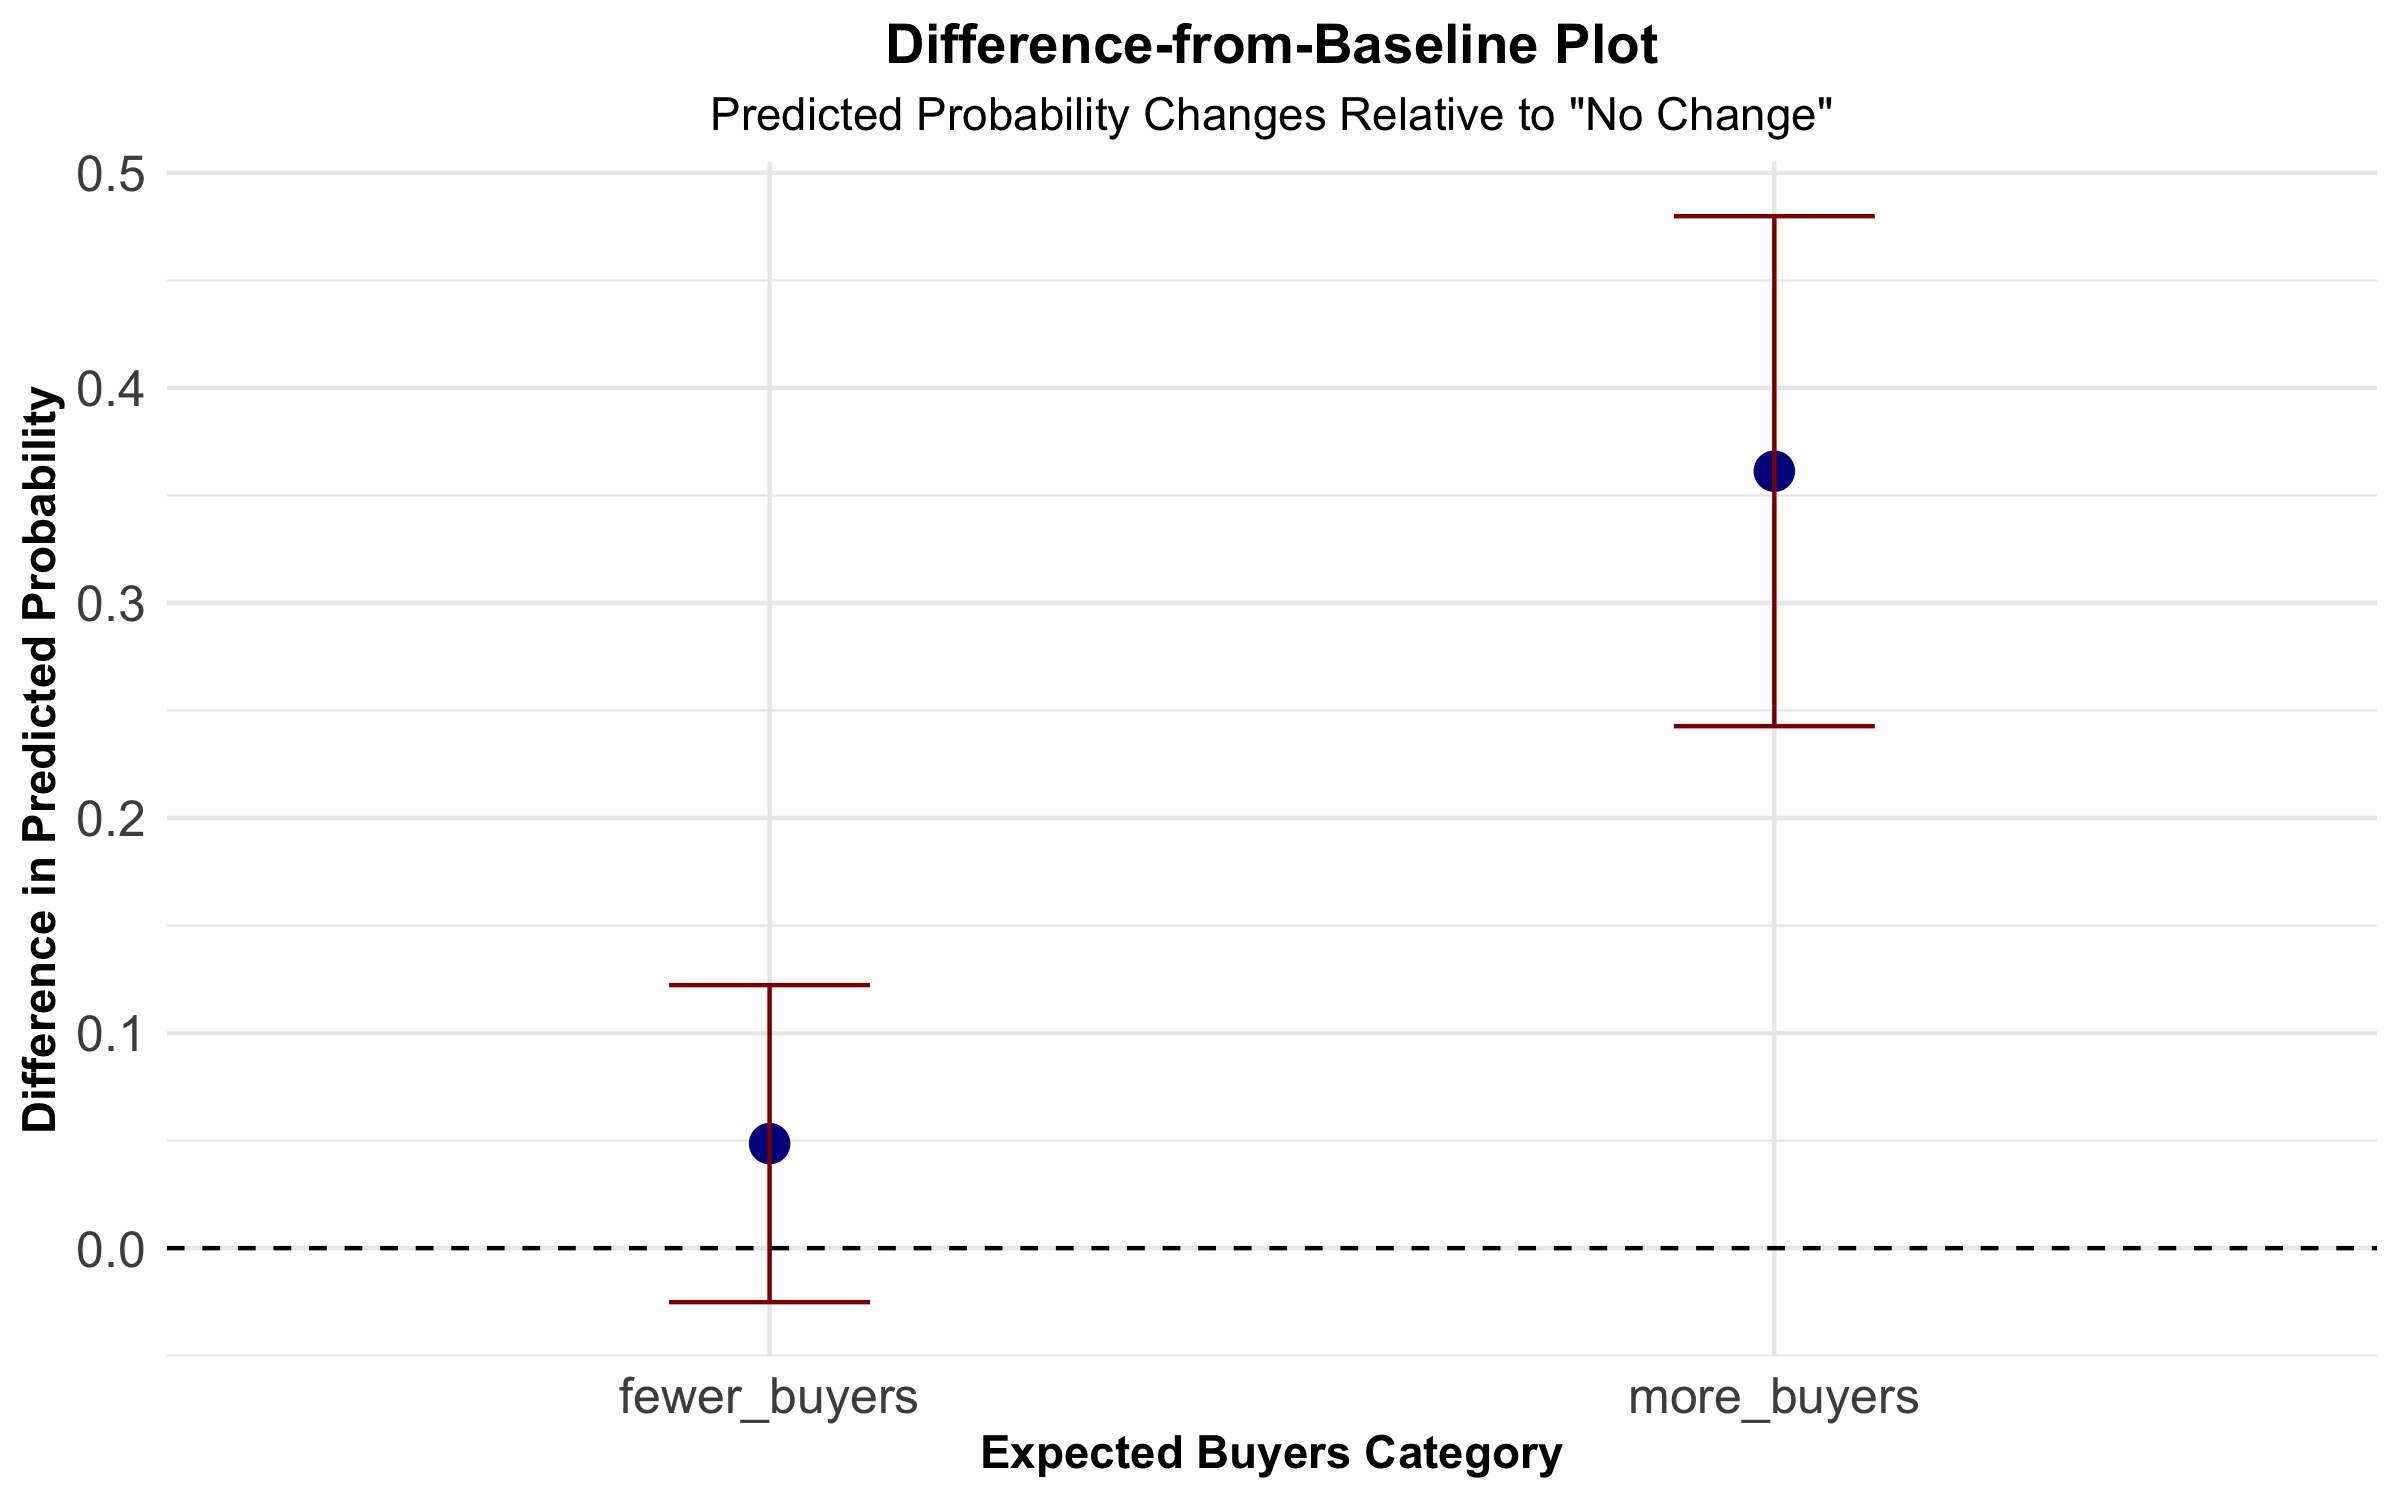
\includegraphics[width=1\textwidth]{figures/filtered_difference_from_baseline_plot.png}
\caption{Difference-from-Baseline Plot}
\label{Figure: Difference-from-Baseline Plot}
\end{figure}

\newpage
\begin{figure}[H]
\centering
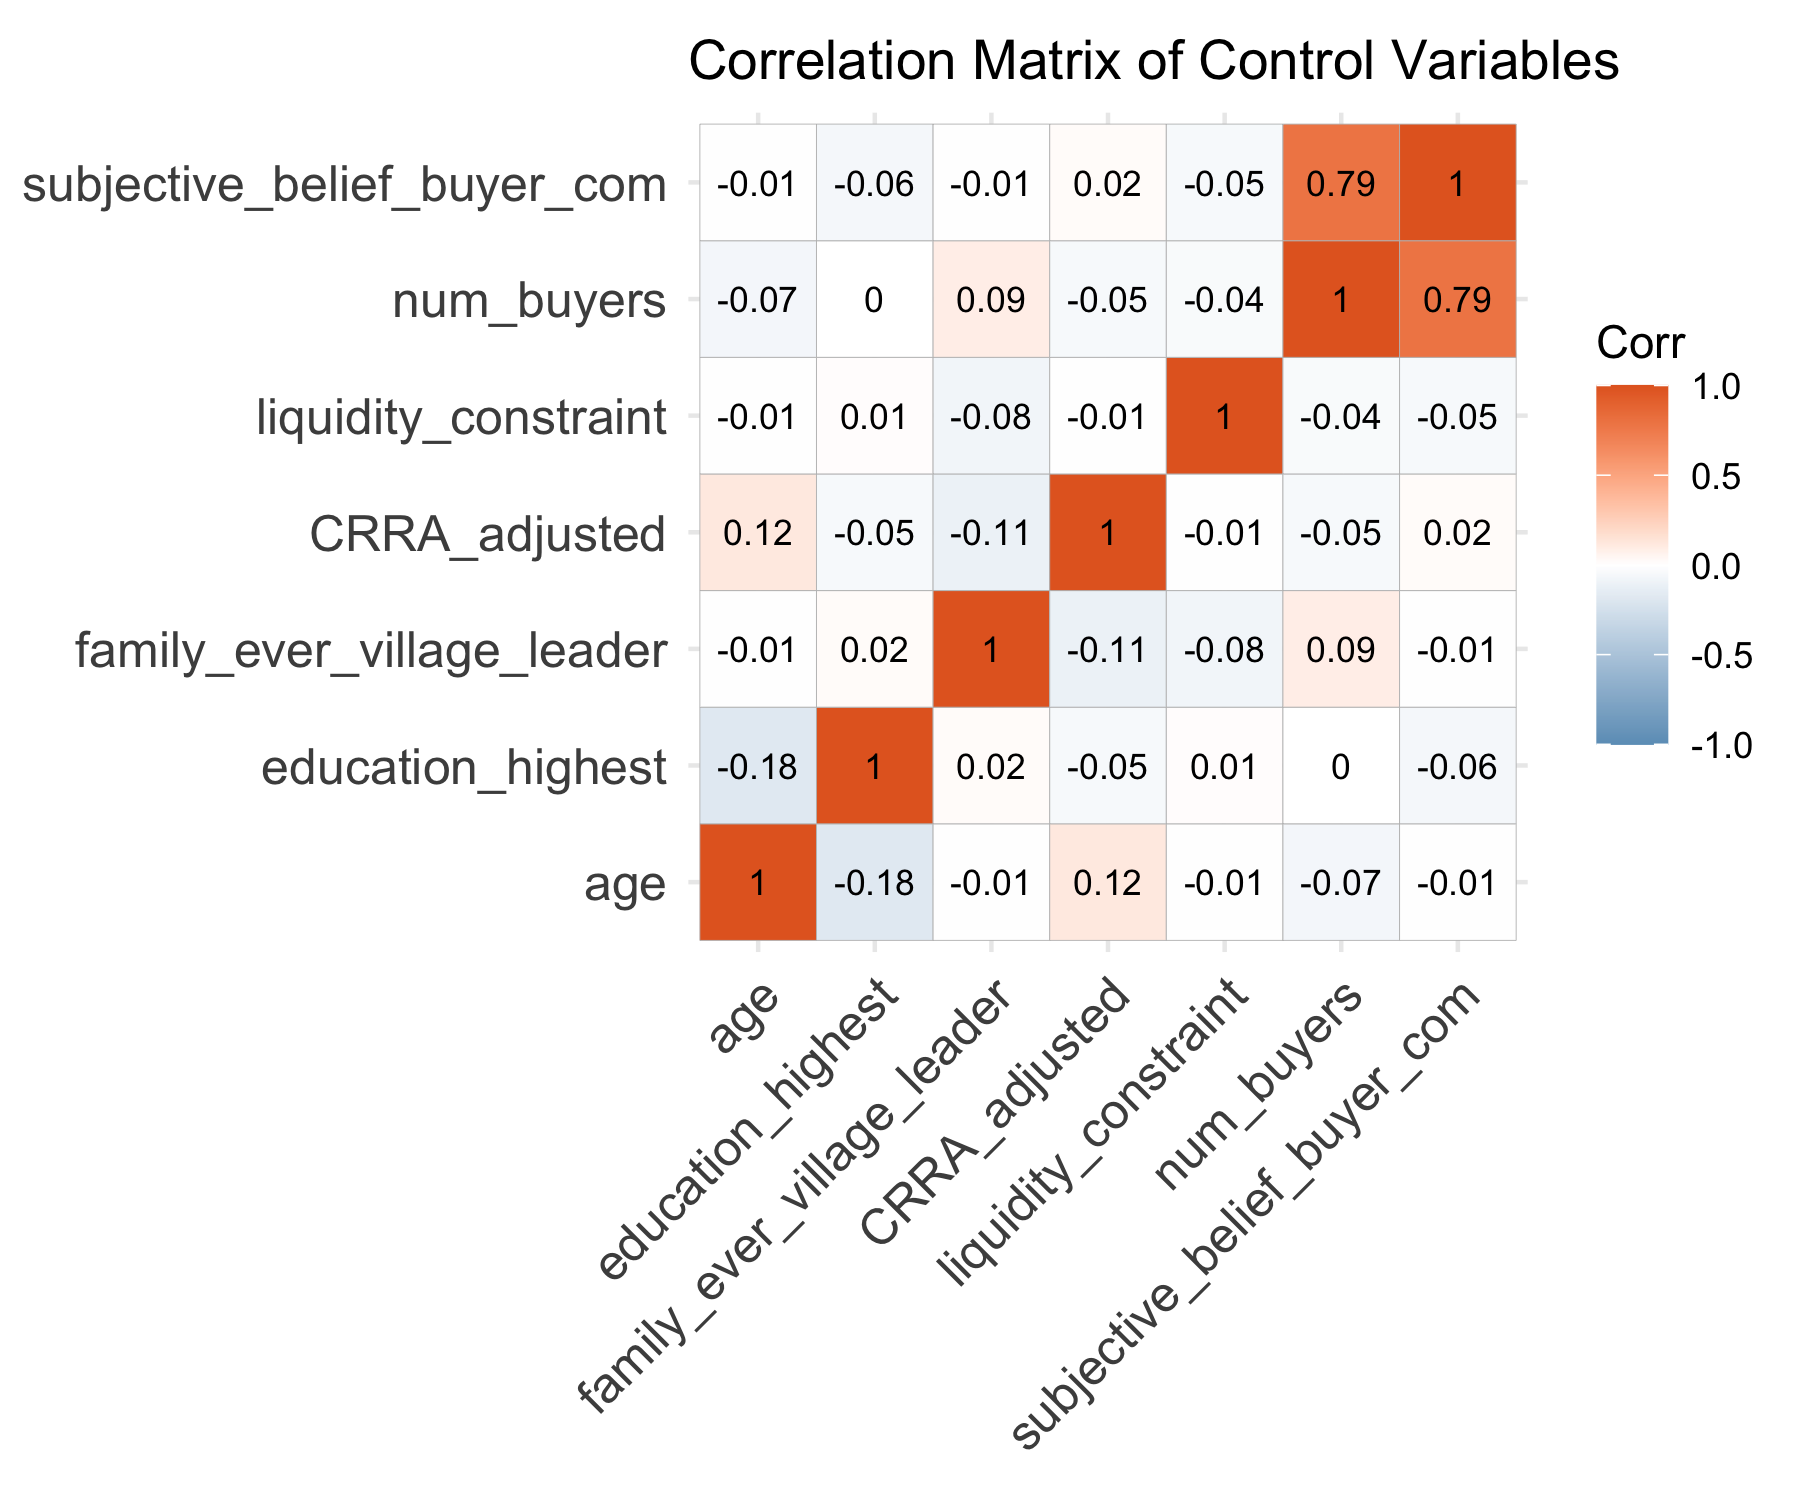
\includegraphics[width=1\textwidth]{figures/correlation_matrix_controls.png}
\caption{Correlation Matrix of Controls}
\label{Figure: Correlation Matrix of Controls}
\end{figure}






\newpage
\subsection{Hazard Models with AFT parametrization}
\subsubsection{Key Concepts and Framework}
Using a hazard model for interval-censored survival data with an accelerated failure-time (AFT) parameterization, like \cite{albuquerque2024market}, we will be able to examine how farmers' expectations of the temporal movement of buyer competitiveness, price expectations, logistical factors, and external conditions influence their marketing timing.

Some concepts are explained below:
\begin{itemize}
    \item Hazard Model: A hazard model, or survival model, can analyze and predict the time until an event of interest occurs. It was firstly developed and applied in disciplines like medicine and public health, which is the origin of its name. 
    \item AFT: AFT parameterization models assume that the effect of covariates is to accelerate or decelerate the survival (marketing/storage in our case) time by a constant factor. For example, a covariate with a positive coefficient may prolong the survival (marketing) time, while a negative effect may shorten it.
    \item Interval censoring: it arises when the event timing is only known to fall within certain bounds. This requires specialized statistical methods to estimate durations and their determinants accurately. 
\end{itemize}



\subsubsection{Hazard Model with AFT Parameterization}
The hazard model describes the likelihood (hazard rate) of selling apples at a specific time, conditional on not having sold them earlier. The AFT framework reinterprets the model by focusing on factors accelerating or delaying the time to sell.

The hazard rate for farmer $f$ selling apples $c$ at time $t_{c,f}$ is:
$$
    h_j(t_{c,f}) = h_0(t_{c,f}) \exp\left(-\mathbf{x}_{c,f} \boldsymbol{\beta}\right),
$$
where we could assume that $h_0(t) = \alpha t^{\alpha-1}$ follows a Weibull distribution, and $\mathbf{x}_{c,f}$ includes explanatory variables.

The survivor function $S_j(t)$, which represents the probability of not selling by time $t$, satisfies $h_j(t) = -\frac{d \log S_j(t)}{dt}. $

For our interval-censored data, the model's likelihood function is:
$$
    \mathcal{L} = \prod_{j=1}^N \left(S_j(t_{i-1}) h(t_i)\right)^{y_{j,i-1}} S_j(t_{i-1})^{1-y_{j,i}},
$$
where $y_{j,i} = 1$ if the sale occurs within the interval $i$.

Our empirical specification includes a township fixed effect to control for unobserved location-specific factors, such as local weather, road conditions, and market infrastructure and access. This township fixed effect improves the model’s ability to account for local heterogeneity but may reduce estimation efficiency due to limited observations within some townships.


\subsubsection{Results}


% Table created by stargazer v.5.2.3 by Marek Hlavac, Social Policy Institute. E-mail: marek.hlavac at gmail.com
% Date and time: Tue, Feb 25, 2025 - 17:32:32
\begin{table}[!htbp] \centering 
  \caption{Weibull Survival Models of Market Timing Decisions} 
  \label{} 
  \resizebox{\textwidth}{!}{%
\begin{tabular}{@{\extracolsep{5pt}}lcccc} 
\\[-1.8ex]\hline 
\hline \\[-1.8ex] 
 & \multicolumn{4}{c}{\textit{Dependent variable:}} \\ 
\cline{2-5} 
\\[-1.8ex] & \multicolumn{4}{c}{lower\_bound\_weeks} \\ 
\\[-1.8ex] & (1) & (2) & (3) & (4)\\ 
\hline \\[-1.8ex] 
 More Buyers Expected & 0.58$^{***}$ & 0.13 &  &  \\ 
  & (0.08) & (0.09) &  &  \\ 
  & & & & \\ 
 Less Buyers Expected & $-$0.04 & $-$0.18$^{*}$ &  &  \\ 
  & (0.07) & (0.11) &  &  \\ 
  & & & & \\ 
 Expected Number of Buyers &  &  & 0.27$^{***}$ & 0.12$^{**}$ \\ 
  &  &  & (0.04) & (0.06) \\ 
  & & & & \\ 
 Constant & 1.55$^{***}$ & 2.14$^{***}$ & 1.66$^{***}$ & 2.12$^{***}$ \\ 
  & (0.07) & (0.11) & (0.07) & (0.09) \\ 
  & & & & \\ 
\hline \\[-1.8ex] 
Town Fixed Effects & Yes & Yes & Yes & Yes \\ 
Observations & 549 & 200 & 549 & 200 \\ 
Log Likelihood & $-$581.66 & $-$287.25 & $-$596.86 & $-$288.39 \\ 
$\chi^{2}$ & 385.18$^{***}$ (df = 9) & 43.19$^{***}$ (df = 8) & 354.77$^{***}$ (df = 8) & 40.93$^{***}$ (df = 7) \\ 
\hline 
\hline \\[-1.8ex] 
\textit{Note:}  & \multicolumn{4}{r}{$^{*}$p$<$0.1; $^{**}$p$<$0.05; $^{***}$p$<$0.01} \\ 
\end{tabular} }
\end{table} 



In the full sample, our Weibull survival estimates indicate that positive market competitive expectations (i.e., anticipating more buyers in the future) are a key driver of longer storage durations (0.499). This suggests that farmers who foresee stronger future demand tend to retain their crops to secure higher prices or more favorable trading terms. By contrast, pessimistic market expectations about future buyers do not significantly affect storage decisions, indicating an asymmetric response where optimism exerts a stronger influence than caution.

Local infrastructure also exerts a prominent effect. The \textit{distance to small storage facilities} has a strong, negative impact on storage duration (-0.301). Farmers located farther from such facilities face higher transport and time costs, which likely discourages them from storing for extended periods. Conversely, \textit{distance to large storage facilities} shows no significant effect, underscoring the importance of proximity to smaller, community-level storage options.

Among the strategic considerations, farmers storing for \textit{broader marketing opportunities} (0.327) or \textit{using storage as a bargaining tool} (0.273) tend to keep their crops longer. Furthermore, education and number of current buyers also increase storage duration (0.100 and 0.029, respectively). These findings suggest that better-informed farmers and those with diverse buyer networks have greater incentives—and the requisite capacity—to store crops until they find more advantageous selling conditions.

In the subsample of dedicated storage users, different patterns emerge. Here, \textit{negative market expectations} about future buyers' competitiveness demonstrate a marginally significant negative effect (-0.211), while positive expectations lose significance. This implies that storage users—likely more risk-averse or heavily invested—are especially sensitive to potential market downturns. Moreover, a \textit{broader buyer network} retains a marginally significant, positive effect on storage duration (0.043), yet strategic motivations such as marketing and bargaining do not yield significant effects within this group. These differences suggest that dedicated storage users might be influenced by factors beyond our current model, including capacity, financing constraints, or established buyer relationships.


% Table created by stargazer v.5.2.3 by Marek Hlavac, Social Policy Institute. E-mail: marek.hlavac at gmail.com
% Date and time: Tue, Feb 25, 2025 - 17:56:36
\begin{table}[!htbp] \centering 
  \caption{Extended Weibull Survival Models with Controls} 
  \label{} 
\begin{tabular}{@{\extracolsep{5pt}}lcc} 
\\[-1.8ex]\hline 
\hline \\[-1.8ex] 
 & \multicolumn{2}{c}{\textit{Dependent variable:}} \\ 
\cline{2-3} 
\\[-1.8ex] & \multicolumn{2}{c}{Full Sample} \\ 
\\[-1.8ex] & (1) & (2)\\ 
\hline \\[-1.8ex] 
 More Buyers Future & 0.50$^{***}$ & 0.12 \\ 
  & (0.07) & (0.09) \\ 
  & & \\ 
 Less Buyers Future & $-$0.05 & $-$0.21$^{*}$ \\ 
  & (0.07) & (0.11) \\ 
  & & \\ 
 Family Village Leader & 0.05 & $-$0.06 \\ 
  & (0.08) & (0.10) \\ 
  & & \\ 
 Far to Small Storage & $-$0.30$^{***}$ & $-$0.14 \\ 
  & (0.07) & (0.10) \\ 
  & & \\ 
 Far to Large Storage & 0.01 & $-$0.13 \\ 
  & (0.10) & (0.15) \\ 
  & & \\ 
 Storage Purpose: Marketing & 0.33$^{***}$ & $-$0.11 \\ 
  & (0.06) & (0.14) \\ 
  & & \\ 
 Storage Purpose: Bargaining & 0.27$^{***}$ & $-$0.05 \\ 
  & (0.06) & (0.11) \\ 
  & & \\ 
 Education Level & 0.10$^{**}$ & 0.06 \\ 
  & (0.04) & (0.07) \\ 
  & & \\ 
 Number of Buyers & 0.03$^{**}$ & 0.04$^{*}$ \\ 
  & (0.01) & (0.02) \\ 
  & & \\ 
 Constant & 1.08$^{***}$ & 2.31$^{***}$ \\ 
  & (0.14) & (0.24) \\ 
  & & \\ 
\hline \\[-1.8ex] 
Town Fixed Effects & Yes & Yes \\ 
Observations & 549 & 200 \\ 
Log Likelihood & $-$527.73 & $-$283.46 \\ 
$\chi^{2}$ & 493.03$^{***}$ (df = 16) & 50.78$^{***}$ (df = 15) \\ 
\hline 
\hline \\[-1.8ex] 
\textit{Note:}  & \multicolumn{2}{r}{$^{*}$p$<$0.1; $^{**}$p$<$0.05; $^{***}$p$<$0.01} \\ 
\end{tabular} 
\end{table} 


\newpage
\bibliography{reference}

\end{document}

